	\documentclass[slidestop,uncompress,mathsans, 12pt]{beamer}
\usepackage[OT1]{eulervm}
%\usepackage[bars]{beamerthemetree}
\usepackage{xcolor}
\usepackage{graphicx}
\usepackage{array}
\usepackage{subfigure}
\usepackage[display]{texpower}
\usepackage{color}
%\usepackage{mathrsfs}
\usetheme{Frankfurt}
\setbeamercolor{alerted text}{fg=red}
%\beamertemplateshadingbackground{blue!5}{yellow!10}
\usecolortheme{whale}
\beamertemplateballitem
%\transglitter[direction=315]

%\useoutertheme{infolines}
%\title[Runzi Qin \space \space \space Rui Guo \space \space \space Yumeng He]{Qin Runzi}
%\subtitle{dsf}
%\institute{Shandong University}
%\date[march 10]{\today}
%\author[Runzi Qin]
\begin{document}
\begin{frame}
\title{Pretend to have a caption}
\subtitle{-----From a Economic Perspective}
\author{Runzi Qin\\   Hongmei Huang\\   Wanyun Hu\\ Jianing Zhang}
\institute{Shandong University}
\titlepage
\end{frame}

\section{Roadmap}
\subsection{Roadmap}
\begin{frame}
\frametitle{Roadmap}
\begin{itemize}
\item Introduction
\item External cause
\begin{enumerate}
\item  Return of Hong Kong
\item  Economic crisis
\item  The rise of mainland China
\end{enumerate}
\item Internal cause
\item  Conclusion
\end{itemize}
\end{frame}
\section{External cause}
\subsection{azi}
\begin{frame}
\title{Return to Hong Kong}
\date{}
\titlepage
\end{frame}
\begin{frame}
\frametitle{Return to Hong Kong}
\begin{itemize}
\item<2-> \alt<2>{\color{blue} Brain drain and capital flight
}{\color{gray} Brain drain and capital flight
}
\bigskip
\item<2-> \alt<3>{\color{blue} Confliction between Hong Kong and mainland
}{\color{gray} Confliction between Hong Kong and mainland
}
\end{itemize}
\end{frame}
\subsection{sdlkfj}
\begin{frame}
\frametitle{Return to Hong Kong}
Brain Drain and Capital Flight\\
\begin{definition}
\textcolor{cyan}{Brain drain}: a mass emigration of technically skilled people from a country or a region to another country. \\
\bigskip
\textcolor{magenta}{Capital flight}: assets or money rapidly flow out of a country or a region, due to an event of economic consequence. \\

\end{definition}
\end{frame}
\begin{frame}
\begin{figure}[h]
\centering
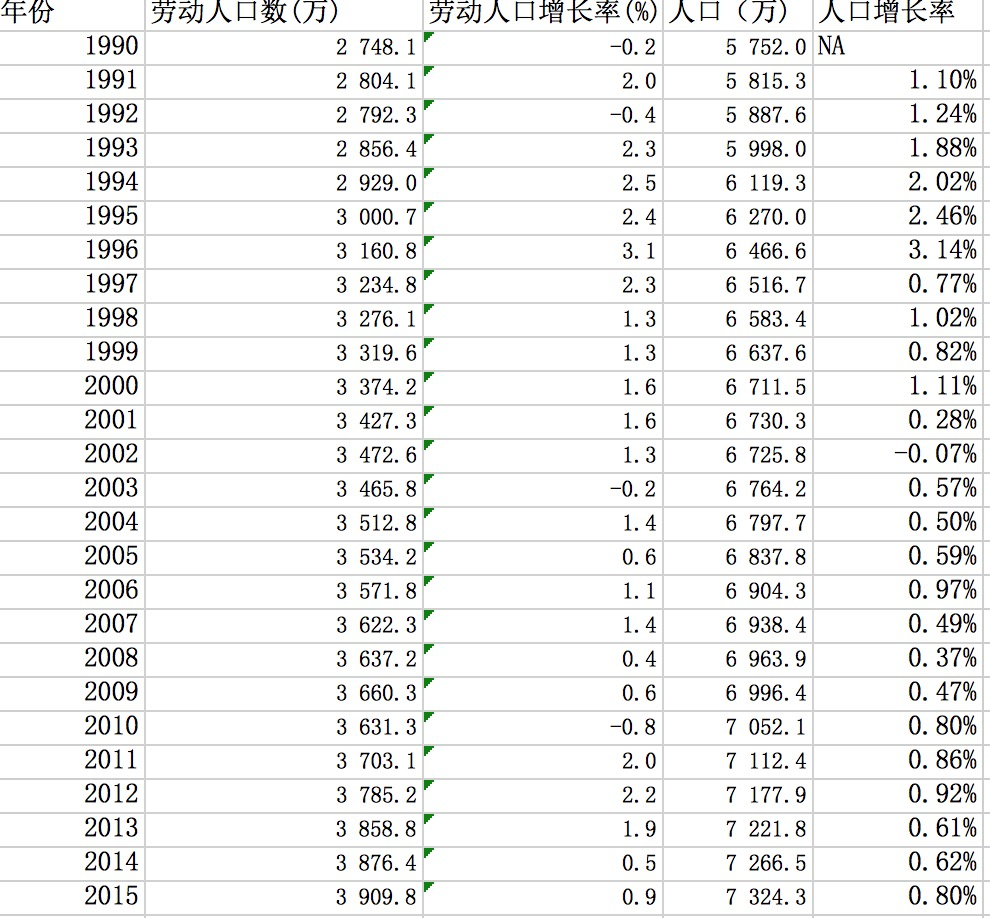
\includegraphics[width=0.8\textwidth]{hk15.jpg}
\label{threadsVsSync}
\end{figure}
\end{frame}
\begin{frame}{Return to Hong Kong}
 Why?
\begin{enumerate}
\item Uncertainty.
\bigskip
\item Better life in other countries.
\end{enumerate}
\end{frame}
\begin{frame}
\frametitle{Return to Hong Kong}
Brain Drain $\Longrightarrow$ Capital Flight
\setbeamercolor{uppercol}{fg=white,bg=blue}%
\setbeamercolor{lowercol}{fg=black,bg=white}%
\begin{beamerboxesrounded}[upper=uppercol,lower=lower col,shadow=true]{Process}
Many capitalists transferred their capital to other countries to avoid the uncertain of Hong Kong and people who emigrated brought their fortune abroad.\\
\end{beamerboxesrounded}
\end{frame}
\begin{frame}{Return to Hong Kong}
Effect
\begin{block}{}
\center{$Y=A \cdot K^a \cdot (EL)^{1-a}$}
\center{$\Downarrow$\\
\bigskip	Economic Downturn}
\end{block}
\end{frame}
\begin{frame}{Return to Hong Kong}
Conflict between Hong Kong and Mainland\\
\bigskip
\bigskip
Institutional difference.\\
\bigskip
\bigskip
Different economic circumstance 

\end{frame}
\subsection{Overview}
\begin{frame}
\title{The Influence of Economic Crisis on Hong Kong }
\date{}
\titlepage
\end{frame}
\begin{frame}[shrink]
\frametitle{The Influence of Economic Crisis on Hong Kong 
}
\begin{itemize}
\item Background
\bigskip
\item Data
\bigskip
\item Explanation
\end{itemize}
\end{frame}
\pageTransitionSplitVI
\subsection{Background}
\begin{frame}

\frametitle{The Influence of Economic Crisis on Hong Kong }
Background\\
\bigskip
\transglitter[direction=315]
On July 2, 1997, Thailand gave up Fixed Exchange Rates, having influence on some countries in Asia.\\
\end{frame}
\begin{frame}
\frametitle{The Influence of Economic Crisis on Hong Kong }
Background\\
\bigskip
On July 2, 1997, Thailand gave up Fixed Exchange Rates, having influence on some countries in Asia.\\
\bigskip
\transboxin<1>
From August 2007, Subprime mortgage crisis spreaded to the whole world which resulted from lending too much to those who are poor in credit.\\
\bigskip
Do they have influence on Hong Kong? Of course yes.
\end{frame}
\subsection{data}
\begin{frame}
\frametitle{The Influence of Economic Crisis on Hong Kong }
Data comes from Hong Kong SAR Government Census and Statistics Department.\\
\bigskip
\begin{figure}[h]
\raggedleft
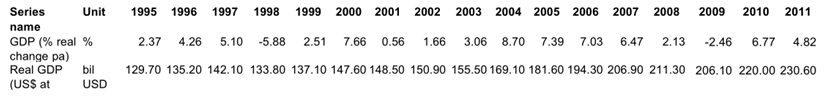
\includegraphics[width=1\textwidth]{hk1.png}
\caption{Data}
\label{threadsVsSync}
\end{figure}
%\begin{table}[htbp]
%\centering  
%\begin{tabular}{ccccccccccccccccccc} 
%\hline
%&Series  %name&Unit&1995&1996&1997&1998&1999&2000&2001&2002&2003
 %&2004&2005&2006&2007&2008&2009&2010&2011\\ \hline  % \hline
% &GDP(\% real change pa)&\%&2.37&4.26&5.10&-5.88&2.51&7.06&0.56&1.66&3.06&8.70&
% &7.39&7.03&6.47&2.13&-2.46&6.77&4.82\\    
% \hline
%\end{tabular}
%\caption{Trade for the last victim: Gaizhen %Wang}
%\end{table}
\end{frame}

\begin{frame}
\frametitle{The Influence of Economic Crisis on Hong Kong }
The real GDP from 1995 to 2011.
\bigskip
\begin{figure}[h]
\raggedleft
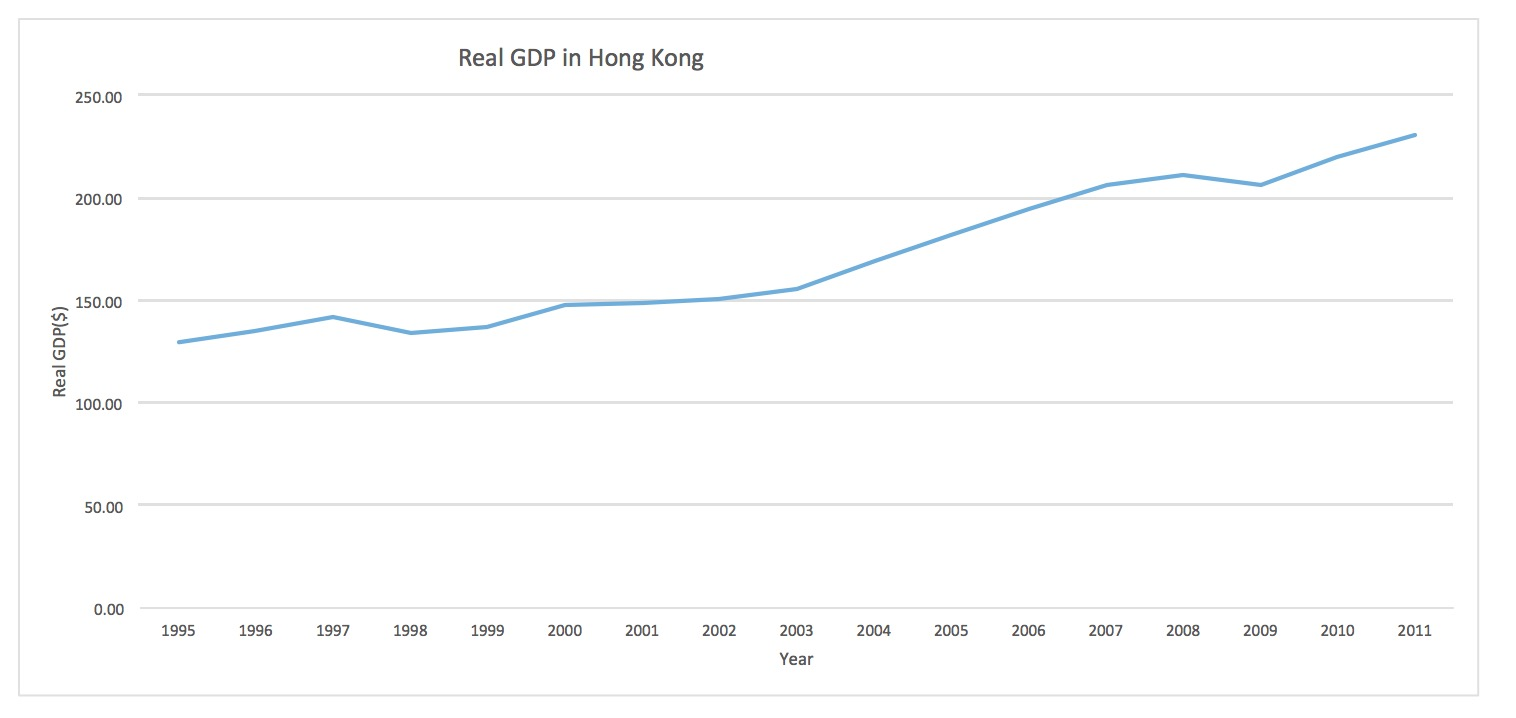
\includegraphics[width=1\textwidth]{hk2.jpg}
\caption{The real GDP}
\label{threadsVsSync}
\end{figure}
\end{frame}

\begin{frame}{The Influence of Economic Crisis on Hong Kong }
GDP growth rate from 1995 to 2011 in Hong Kong.\\
\bigskip
\begin{figure}[h]
\raggedleft
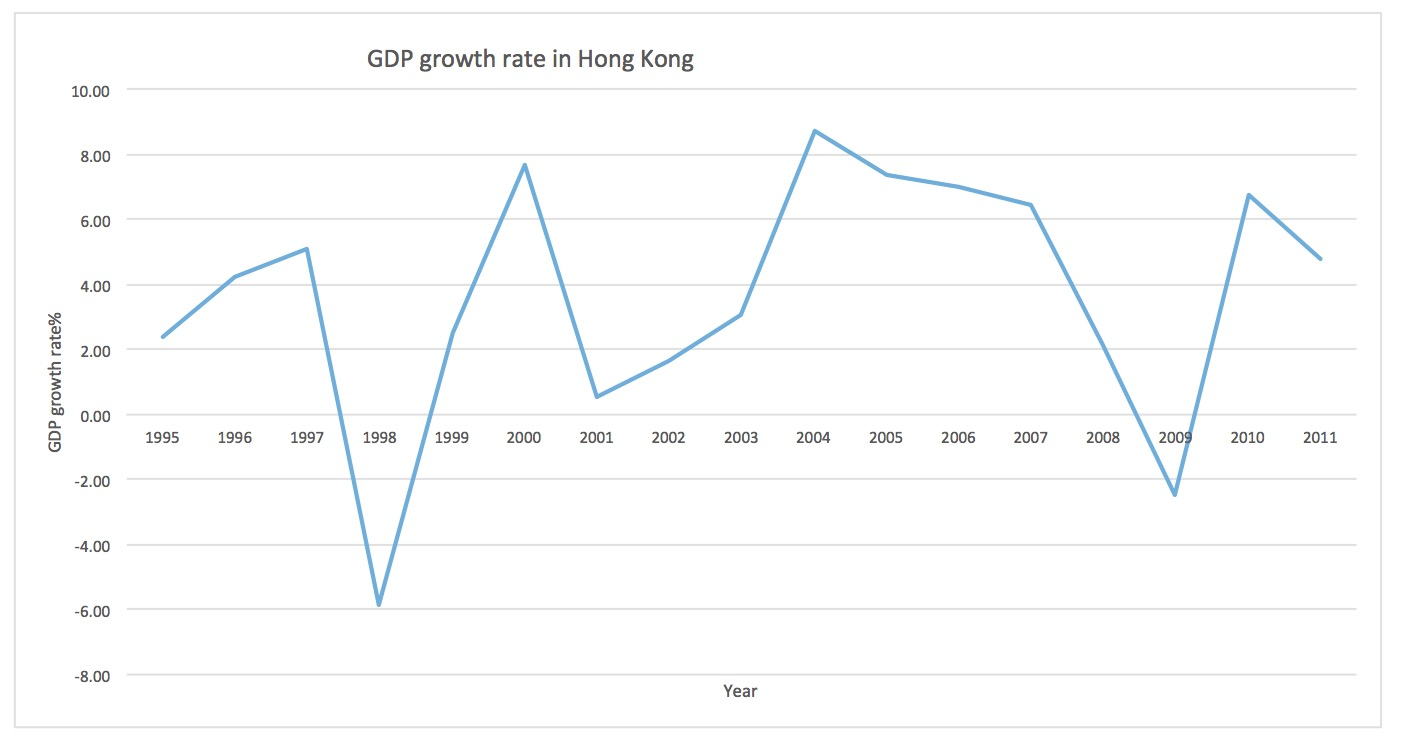
\includegraphics[width=1\textwidth]{hk3.jpg}
\caption{GDP growth rate}
\label{threadsVsSync}
\end{figure}
\end{frame}

\subsection{Explanation}
\begin{frame}{The Influence of Economic Crisis on Hong Kong }
Explanation\\
\bigskip
\alert{Financial Crisis in 1997}
\bigskip

\begin{enumerate}[i]
\pause\item Thailand gave up Fixed Exchange Rates causing foreign exchange market chaotic.
\bigskip
\pause\item International speculators began to “attack” Hong Kong in October 1997 and another “attack” in August 1998.
\bigskip
\pause\item In reaction, government must increase interest rate which makes the stock market sharply fall. In addition, they sell foreign exchange reserve to stablize the exchange rate causing it decrease.
\bigskip
\pause\item A panic appeared in Financial market, causing less investment.
\end{enumerate}

\end{frame}

\begin{frame}
\frametitle{The Influence of Economic Crisis on Hong Kong }
Explanation\\
\bigskip
\alert{Financial Crisis in 1997}
\bigskip
\begin{enumerate}[I]
\item <+-| alert@+> Subprime crisis. 
\bigskip
\item <+-| alert@+> Panic in the market, causing currency less liquid. The world economy came into recession.
\bigskip
\item <+-| alert@+> Hong Kong being a part of economy can't escape. 

\bigskip

\end{enumerate}
\end{frame}
\subsection{Huang}
\begin{frame}
\title {The Impact of The Rise of China's Economy on Hong Kong's Economic Status}
\date{}
\titlepage
\end{frame}
\begin{frame}{The Rise of Chinese Economy}
Roadmap\\
\begin{itemize}
\item Hong Kong's special economic status for China\\
\item The Rise of China's economy\\
\item The impact on Hong Kong's economic status\\

\end{itemize}

\end{frame}
\begin{frame}
\frametitle{The Rise of Chinese Economy}
The Special Economic Status of Hong Kong\\
\bigskip
\animate<1-4>%
\begin{itemize}[<+->]
\item The leading economic zone: “Dragon's Head”.
\item The mediation role on investment, capital introduction and the processing trade.
\item The financial center: provide offshore financial services.
\item The political reason.
\end{itemize}
\pause
\end{frame}

\begin{frame}
\frametitle{The Rise of Chinese Economy}
The reason of the Special Status\\
\bigskip
\begin{enumerate}[A]
\item The high economic density.
\bigskip
\item The close economic relationship.
\bigskip
\item The multiple advantages of Hong Kong's economy.
\end{enumerate}
\end{frame}

\subsection{High Density}
\begin{frame}
\frametitle{The Rise of Chinese Economy}
The High Economic Density\\
\bigskip
\bigskip
\begin{figure}[h]
\raggedleft
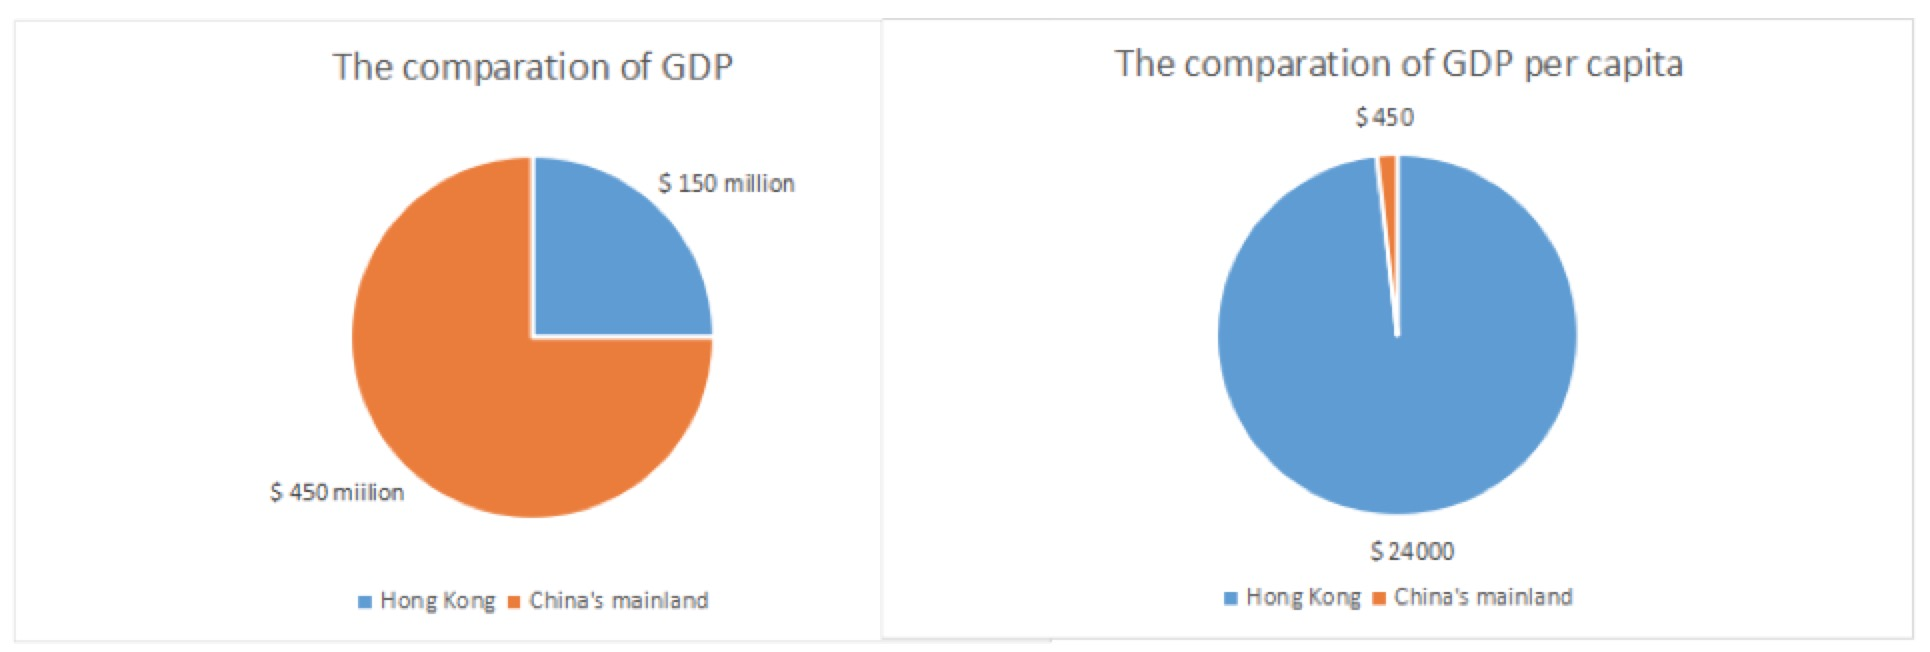
\includegraphics[width=1\textwidth]{hk5.jpg}
\label{threadsVsSync}
\end{figure}
\flushright{Shanghai \$$3000$}
\end{frame}

\subsection{close relationship}
\begin{frame}{The Rise of Chinese Economy}
The Close Economic Relationship\\
\bigskip
The economic return runs before the political return. \\
\begin{overprint}
\onslide<1>

\begin{figure}[h!]
\centering
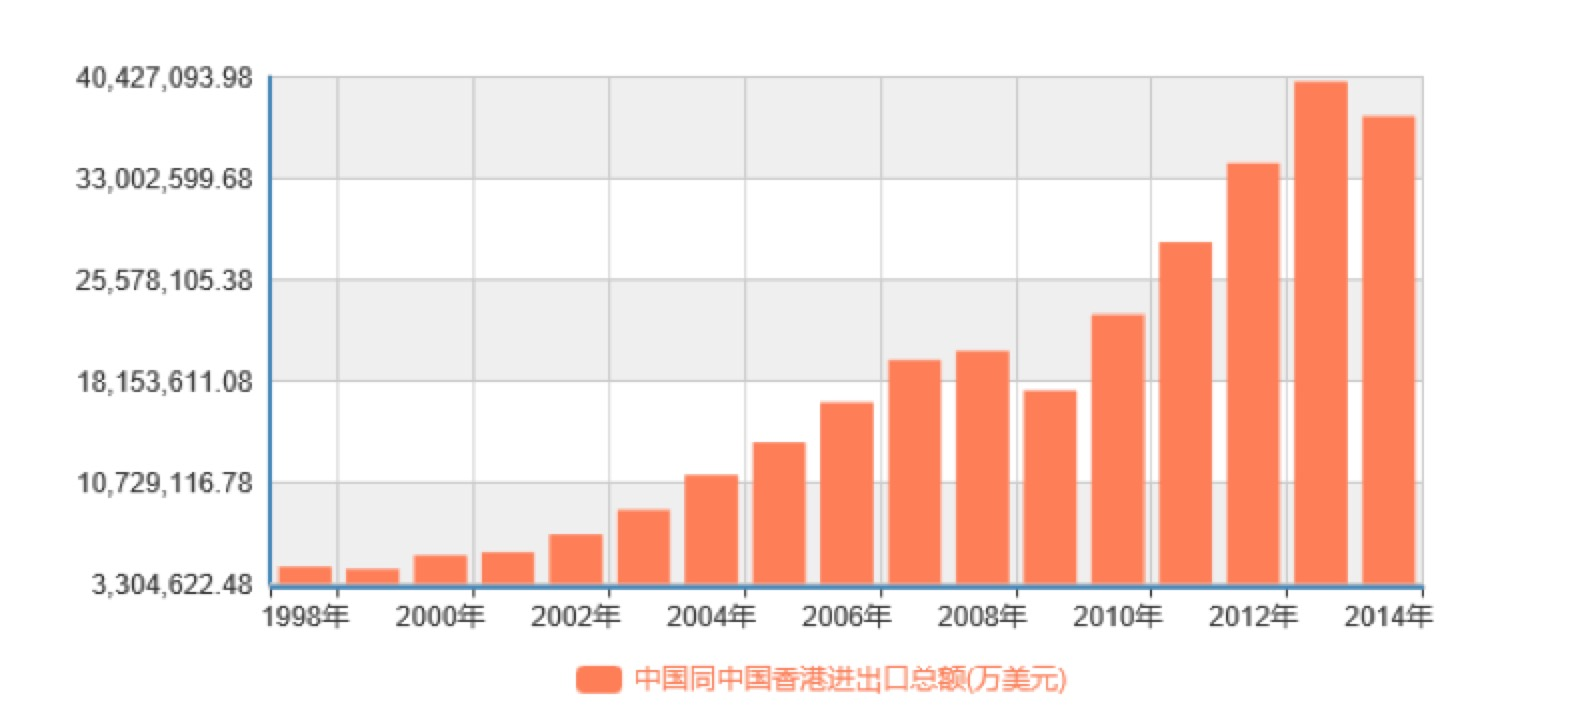
\includegraphics[width=1.05\textwidth]{hk6.jpg}
\label{threadsVsSync}
\end{figure}
\onslide<2>
Case: In 1980s,  the north movement of manufacture industries contributed to the economic development of Guangdong.\\ 
\begin{figure}[h!]
\centering
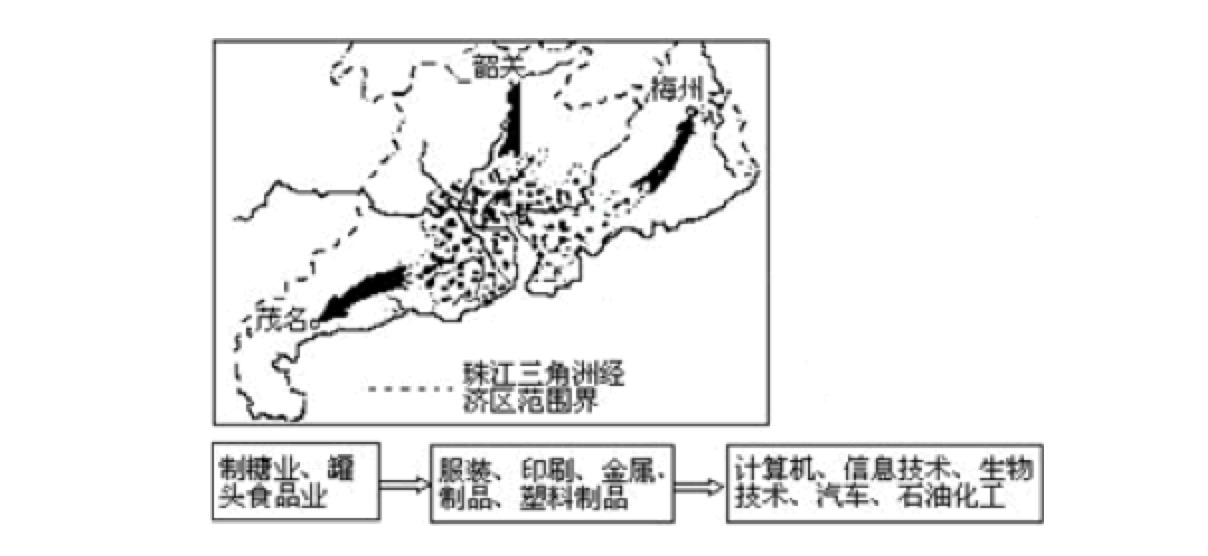
\includegraphics[width=0.7\textwidth]{hk7.jpg}
\label{threadsVsSync}
\end{figure}
\end{overprint}
\end{frame}

\begin{frame}
\frametitle{The Rise of Chinese Economy}
Advantages of Hong Kong's Economic\\
\bigskip
\begin{enumerate}
\item The complete economic policy system.
\bigskip
\item The high economic freedom.
\bigskip
\item The service industry-dominated structure.
\bigskip 
The prosperity of finance, information, transportation, international trade.
\end{enumerate}

\end{frame}
\subsection{Rise}
\begin{frame}
\frametitle{The Impact of The Rise of China's Economy on Hong Kong's Economic Status}
The rise of China's Economy\\
An economic miracle.\\
\bigskip
\begin{figure}[h!]
\centering
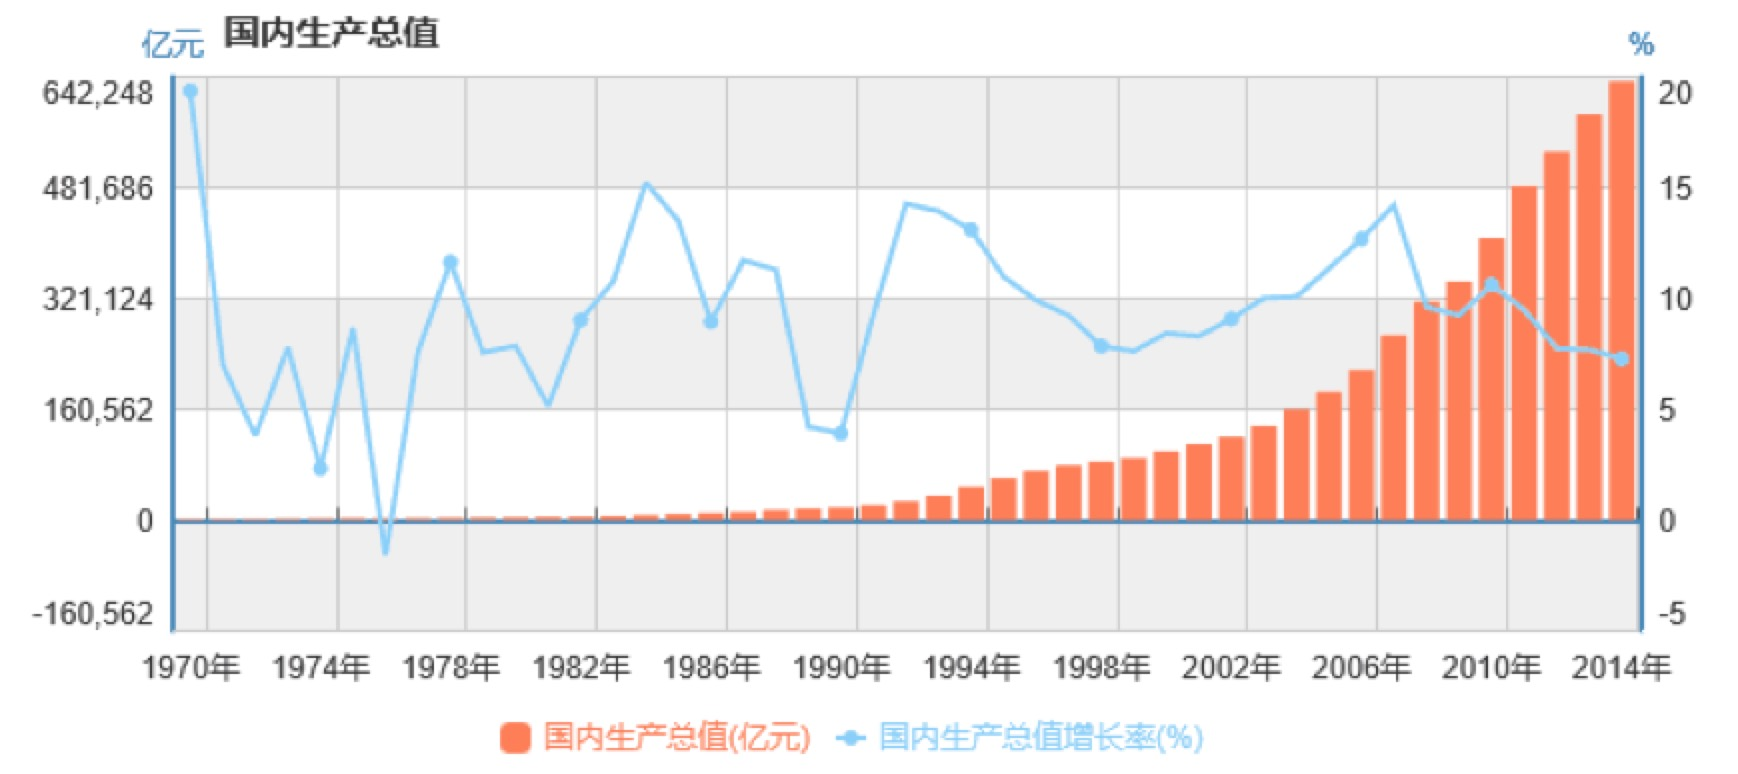
\includegraphics[width=1\textwidth]{hk8.jpg}
\label{threadsVsSync}
\end{figure}
\end{frame}



\begin{frame}
\frametitle{The Rise of Chinese Economy}
The rise of economic zones like Beijing, Shanghai and    Shenzhen. \\
\begin{figure}[h!]
\centering
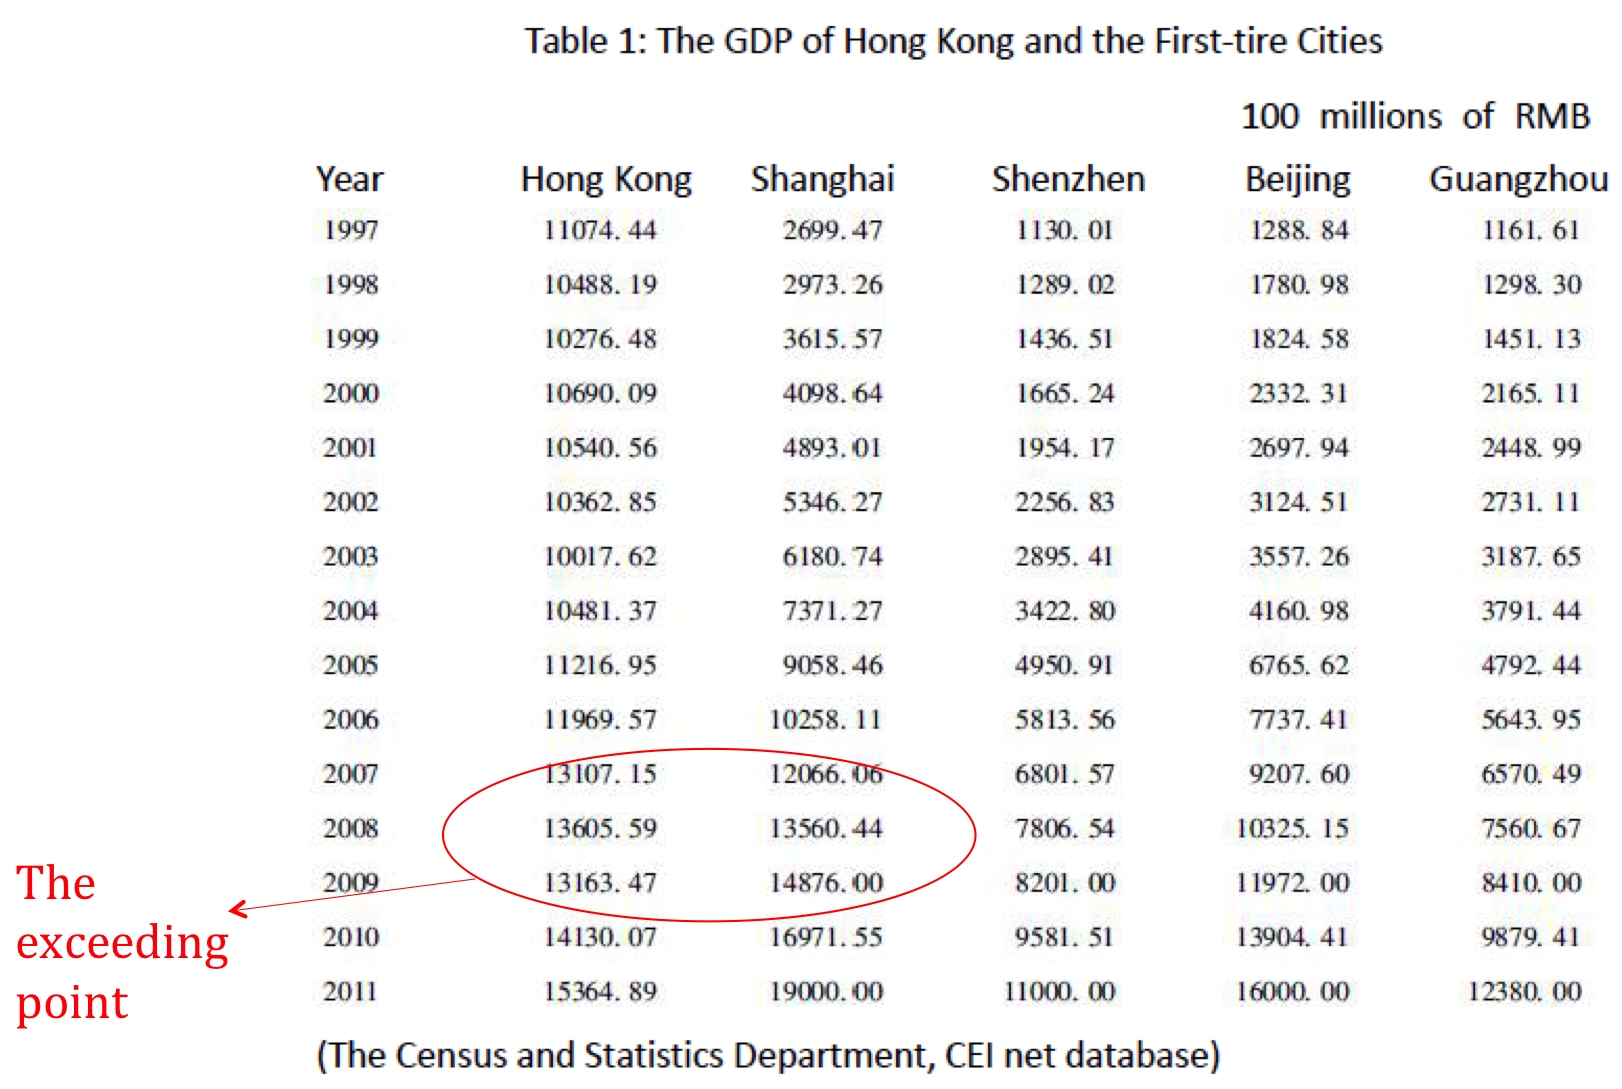
\includegraphics[width=0.7\textwidth]{hk8.png}
\label{threadsVsSync}
\end{figure}
\end{frame}
\begin{frame}{The Rise of Chinese Economy}
The impact on Hong Kong's economic status\\
\bigskip
From the perspective of the background of Hong Kong's rise\\
\bigskip
\bigskip
Shanghai financial center went to the weak
$\Longrightarrow$ the rise of Shanghai, Beijing and Shenzhen\\
\bigskip
\bigskip
The economic autarky situation, the planned economy
$\Longrightarrow$ The more open economy, the maket economy.\\
\bigskip
\bigskip
The lack of bridge between China and foreign coutries
$\Longrightarrow$ The second largest international trade country.\\
 



\end{frame}
\subsection{The impact on Hong Kong's economic status}
\begin{frame}
\frametitle{The Rise of Chinese Economy}
The impact on Hong Kong's economic status\\
\bigskip
From the perspective of the institutinal reasons\\
\bigskip
Government's policy change.\\
\bigskip
Political institutional contradiction.\\
\bigskip
Different economy system on tax, trade, accounting policy.
\end{frame}
\begin{frame}
\frametitle{The Rise of Chinese Economy}
The impact on Hong Kong's economic status\\
\bigskip
From the perspective of the institutinal reasons\\
\bigskip
Government's policy change.\\
\bigskip
Political institutional contradiction.\\
\bigskip
Different economy system on tax, trade, accounting policy.
\end{frame}
\begin{frame}{The Rise of Chinese Economy}

\transwipe<1>
The impact on Hong Kong's economic status\\
\bigskip
From the perspective of the cultural reasons.\\
\bigskip
The Hong Kong’s native consciousness.\\
\bigskip
The worship of British.\\

\end{frame}
\section{Internal cause}
\subsection{competitive}
\begin{frame}

\title{The Economic Competitiveness of Hong Kong}
\date{}
\titlepage
\end{frame}
\begin{frame}
\frametitle{The Economic Competitiveness of Hong Kong}
\transdissolve<1>
a.The competitiveness ranking of Hong Kong
We referenced the Global Competitiveness Report produced by World Economic Forum, and figured the competitiveness ranking of Hong Kong.
\\

\begin{figure}[h]
\raggedleft
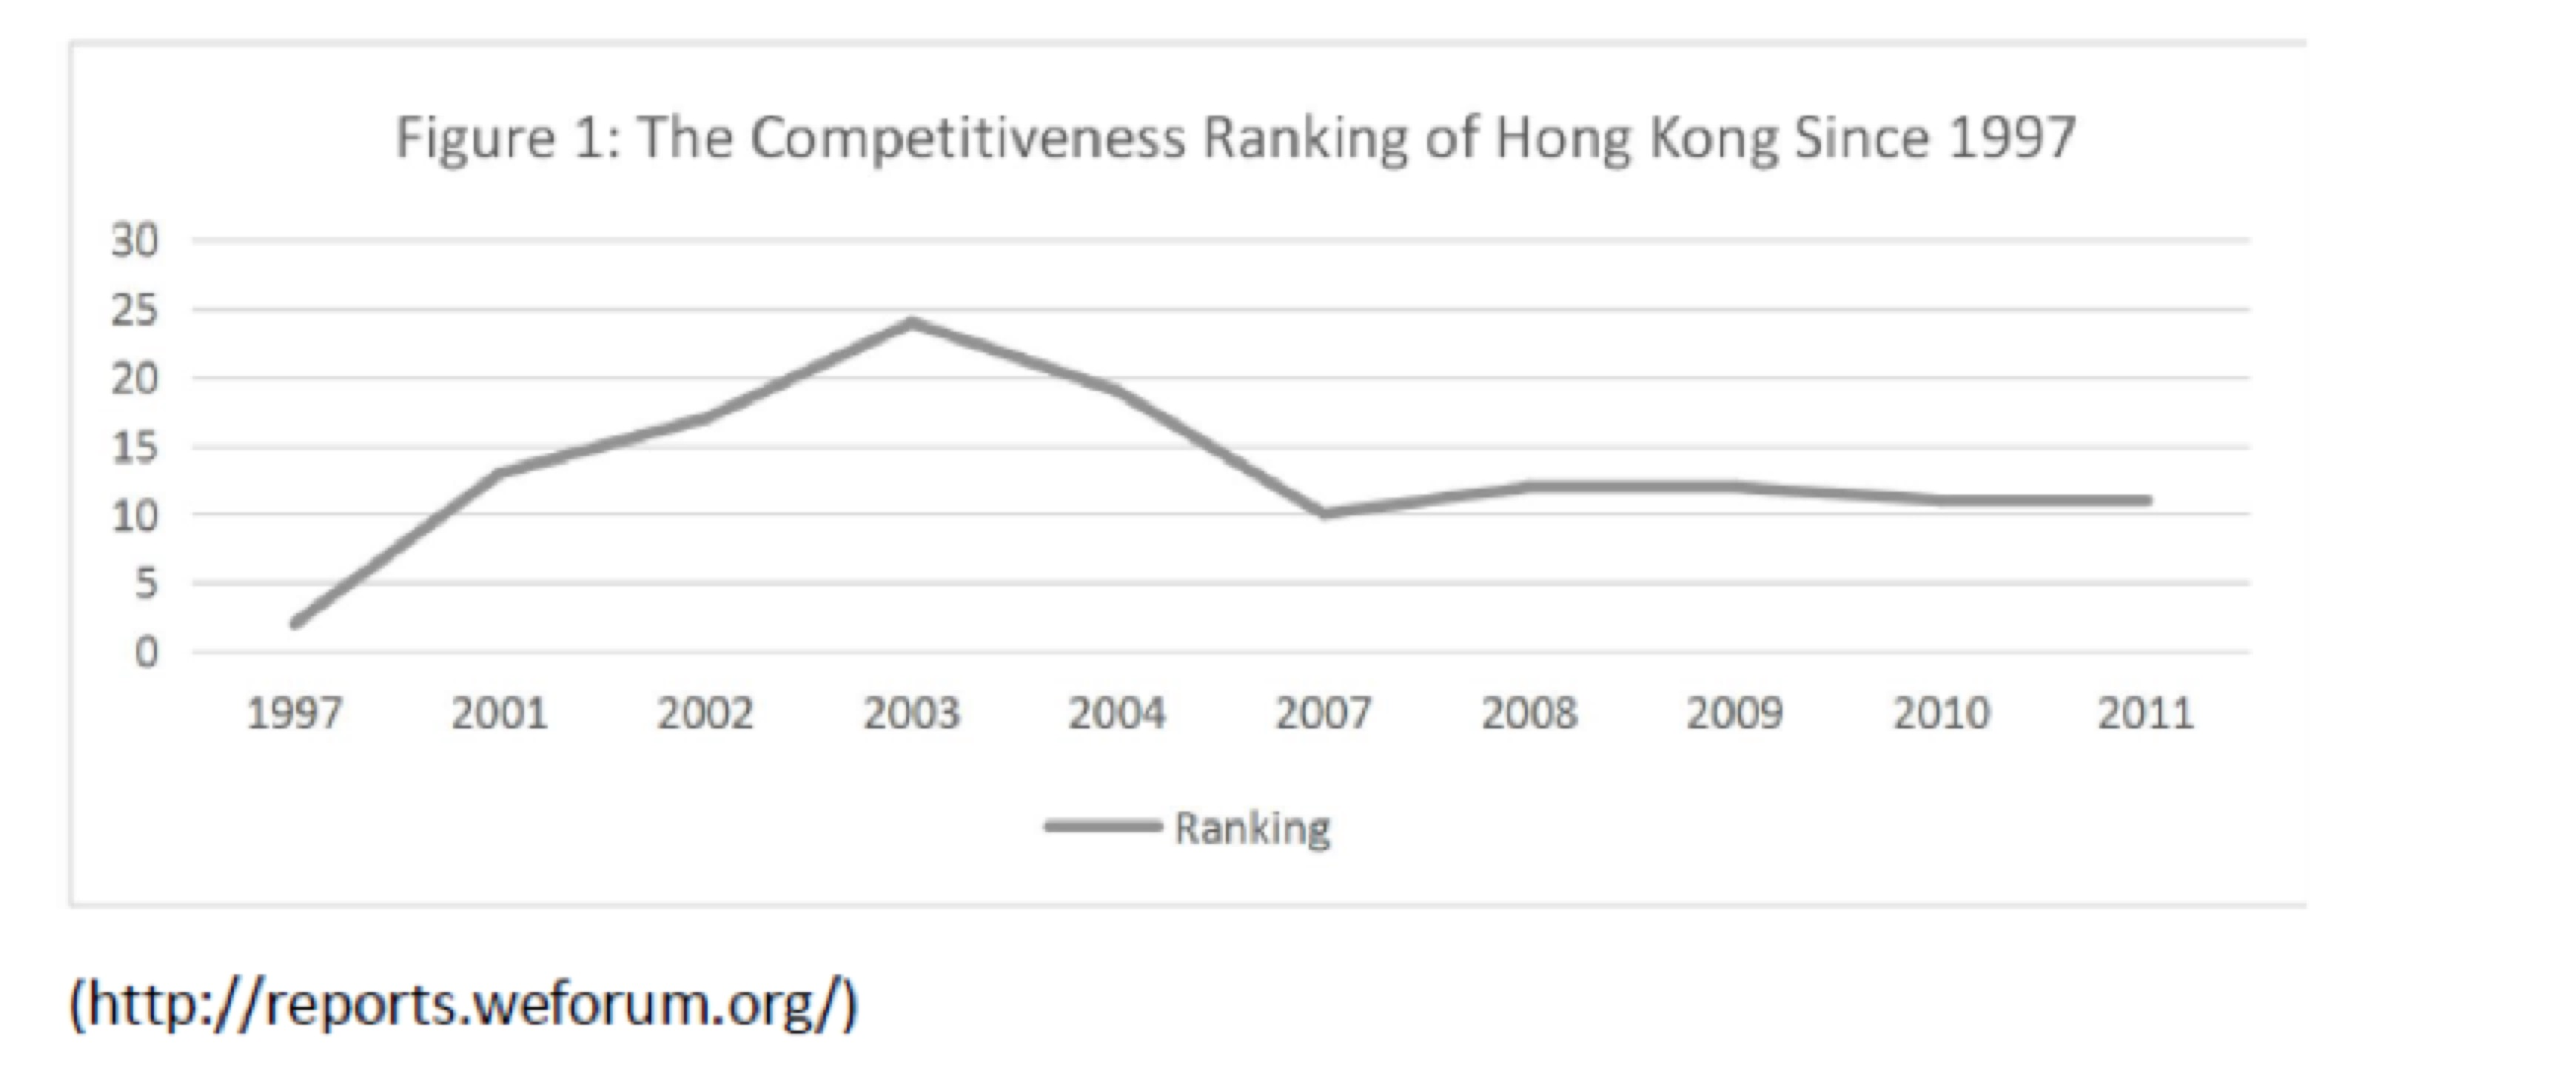
\includegraphics[width=1.1\textwidth]{hk4.jpg}
\label{threadsVsSync}
\end{figure}
\end{frame}
\begin{frame}[shrink]
\frametitle{The Economic Competitiveness of Hong Kong}
b.  The economic position of Hong Kong in the Chinese economic territory
It can be seen that the economic position of Hong Kong is relatively decreasing in the Chinese economic territory. And the economic competitiveness of Hong Kong is also relatively decreasing.\\
\begin{figure}[h]
\raggedleft
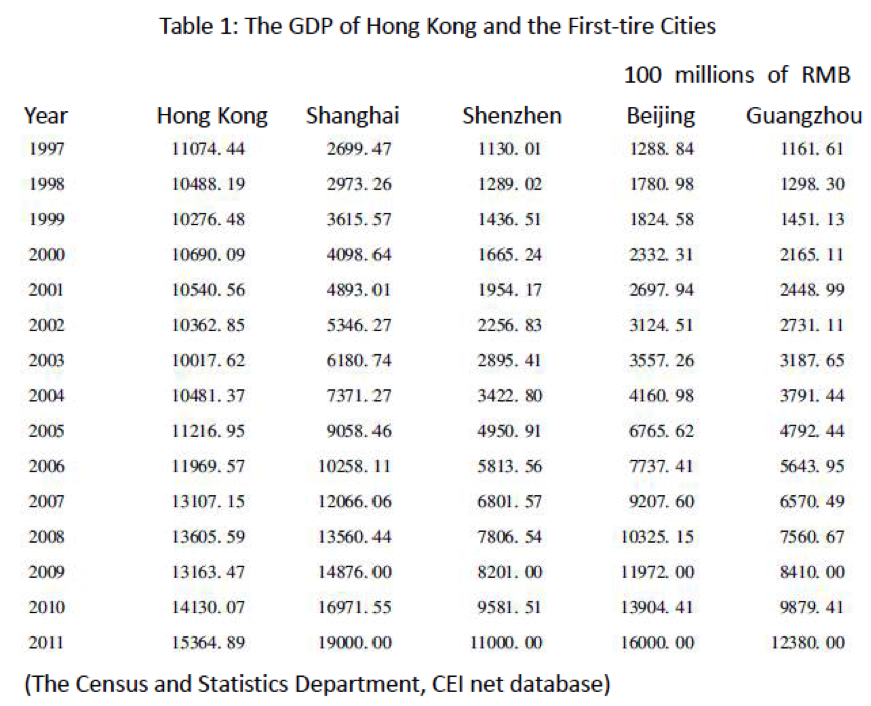
\includegraphics[width=0.6\textwidth]{hk9.png}
\label{threadsVsSync}
\end{figure}
%\begin{table}[htbp]
 
%\begin{tabular}{ccccc} 
%\hline
 %&1%$^{st}$ Stage&2$^{st}$ Stage&$\cdots$&4$^{st}$ %Stage\\ \hline  % \hline
 %&TianTang Song &Qiaoling Zhang
%5& &Ultimate Buyer\\    \hline      
%Price &3,000RMB &7000RMB & &14,000RMB\\        \hline
%\end{tabular}
%\caption{Trade for the last victim: Gaizhen Wang}
%\end{table}
\end{frame}
\begin{frame}
\frametitle{The Economic Competitiveness of Hong Kong}%[shrink]
c. The financial market of Hong Kong
And according to Levine (2000) and Arestis (1997), we use the M2/GDP, Loan/M2, Stock market value/GDP to present the competitiveness of Hong Kong financial market.\\
\begin{overprint}
\onslide<1>
\begin{figure}[h]
\centering
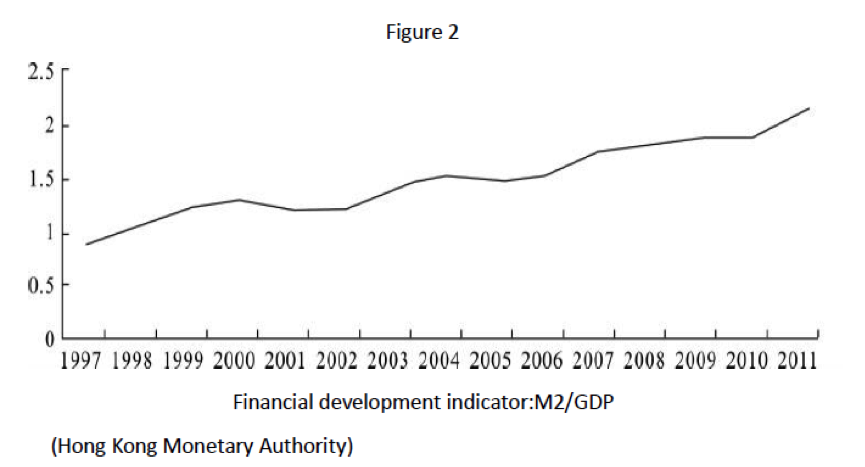
\includegraphics[width=1\textwidth]{hk10.png}
\label{threadsVsSync}
\end{figure}
\onslide<2>
\begin{figure}[h]
\centering
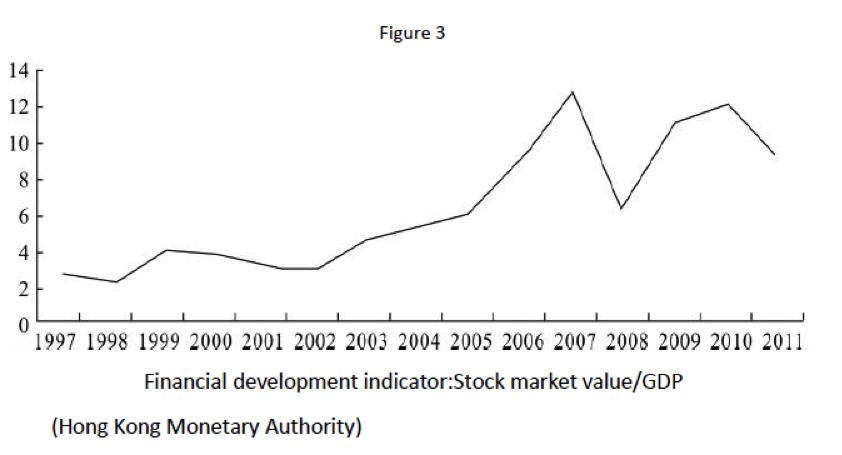
\includegraphics[width=1\textwidth]{hk11.png}
\label{threadsVsSync}
\end{figure}
\onslide<3>
\begin{figure}[h]
\centering
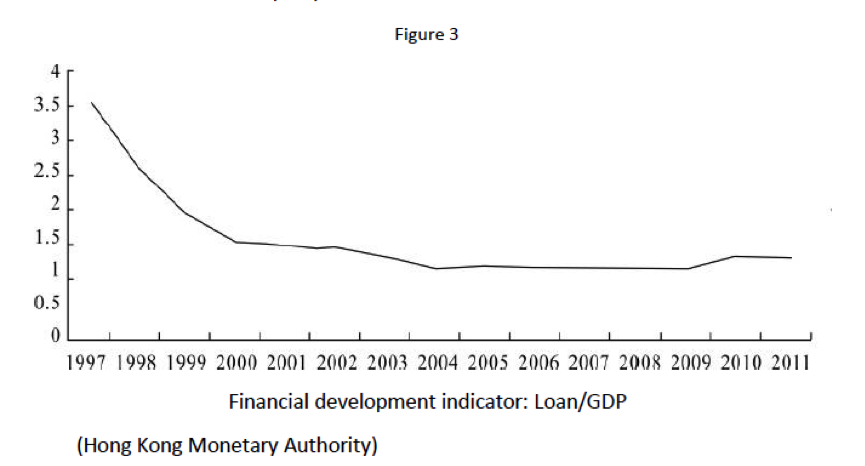
\includegraphics[width=1\textwidth]{hk12.png}
\label{threadsVsSync}
\end{figure}
\end{overprint}
\end{frame}
\begin{frame}
\frametitle{The Economic Competitiveness of Hong Kong}
d.  Trade and logistics of Hong Kong\\
\begin{figure}[h]
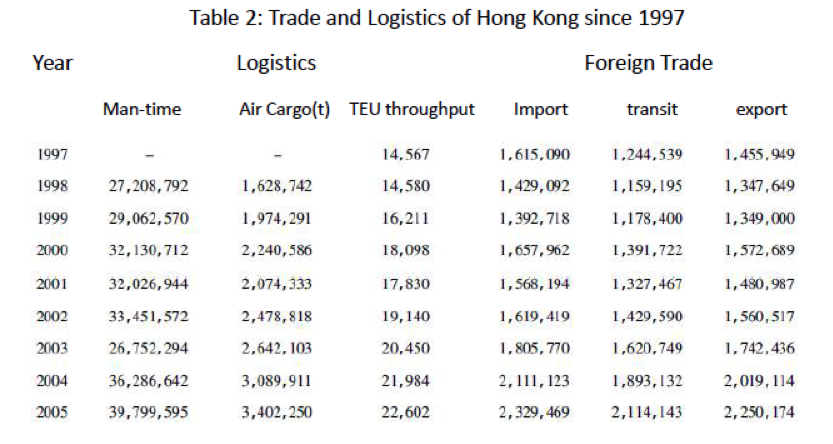
\includegraphics[width=0.6\textwidth]{hk13.png}
\label{threadsVsSync}
\end{figure}
\begin{figure}[h]
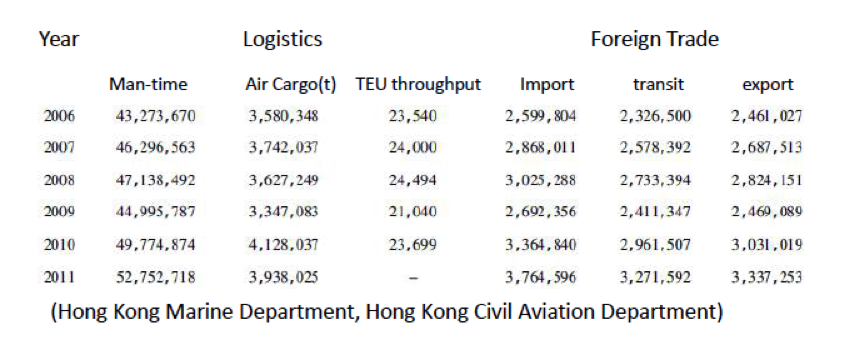
\includegraphics[width=0.6\textwidth]{hk14.png}
\label{threadsVsSync}
\end{figure}
\end{frame}
\section{Conclusion}
\begin{frame}{Conclusion}

\bigskip
\bigskip

\begin{block}{\center{Conclusion}}
Pretend to have a conclusion.
\end{block}
\end{frame}
\begin{frame}
\transsplitverticalin<1>
\bigskip
\bigskip
\bigskip
\bigskip
\bigskip
\bigskip
\bigskip
\bigskip

\center{$\mathcal{THANK}$}\\ 
\center{$\mathcal{YOU}$}
\end{frame}
\end{document}
